\section{Experiments: initialization, geometry and stopping}
\label{sec:experiments}
The experiments test finite-budget behavior rather than tightness of the
worst-case constants. All methods use the same scalar certificate unless
a stopping control is explicitly identified. We distinguish function,
gradient and full LMO budgets; no arbitrary conversion weights or
wall-clock ranking are imposed. AFW active-set scans and atom scores
are recorded separately. Capped runs remain in summaries.

\subsection{Count-data objectives with verified curvature bounds}
The main real-data protocols use Seoul Bike Sharing Demand~\cite{seoul}
and Metro Interstate Traffic Volume~\cite{metro}, with the unmodified
official files, hashes and CC BY 4.0 attribution retained. A stable
chronological sort and the first 80\% of rows define training data.
Non-intercept features are transformed by
$\tanh((v-\bar v_{\rm train})/s_{\rm train})$, using training statistics
only; an intercept is included and constrained. Repeated source
timestamps keep their original weights. We optimize a training
objective, not a predictive-performance criterion.

With normalized response $t_i=y_i/\bar y_{\rm train}$ and
$c_i=t_i\log t_i-t_i$ (with $0\log0=0$), the objective is
\begin{equation}\label{eq:poisson}
 f(x)=\frac1m\sum_i\{e^{a_i^\top x}-t_i a_i^\top x+c_i\}
          +\frac{\mu}{2}\norm x^2,\qquad \norm x_1\le R,
 \quad\mu=0.01.
\end{equation}
All coordinates, including the intercept, are ridge-regularized.
Since $\norm{a_i}_\infty=1$ and $\operatorname{mean}(t_i)=1$, valid
constants relative to the constrained optimum are
\begin{equation}\label{eq:poissonconstants}
 H_1=\max_i\norm{a_i}^2,\qquad H_0=\mu+H_1(1+R),\qquad
 L_Q=\mu+e^R\lambda_{\max}(A^\top A/m).
\end{equation}
The Hessian norm is at most $\mu+H_1\operatorname{mean}(e^{a_i^\top x})$.
Since $f_Q^*\le f(0)$, the objective formula gives
\[
 \operatorname{mean}(e^{a_i^\top x})\le\delta+1+R.
\]
These are analytic upper bounds, not fitted or minimal constants.
On a compact domain a global Lipschitz bound also exists.

\begin{table}[htbp]
\centering\small
\caption{Count-data protocols. $R_*$ is the offline unconstrained reference $\ell_1$ norm; tested radii are $R_*/2$ and $2R_*$. Widths are numerical reference brackets, without directed rounding. All $2d$ signed coordinate vertices are used at each radius.}
\label{tab:data}
\begin{tabular}{lrrrrr}
\toprule
Data & Training rows & $d$ & $R_*$ & $H_1$ & Max. width \\
\midrule
Seoul & 7008 & 15 & 4.575821 & 8.897 & 4.2e-08 \\
Metro & 38563 & 12 & 1.431745 & 6.208 & 2.3e-09 \\
\bottomrule
\end{tabular}
\end{table}

An offline damped Newton reference estimates
$R_*=\norm{x^*_{\rm unc}}_1$.
The radii $R_*/2$ and $2R_*$ give active and interior controls, with
independently recomputed constrained numerical references.
Each reference uses a feasible value as an upper bound and its convex
tangent/LMO lower bound. These are numerical brackets without directed
rounding, not formal interval certificates. They are never solver inputs.
We report post-run error bounds to this numerical precision.
All $2d$ signed coordinate vertices are used once at each radius:
108 dataset/radius/start cases in total. Radii and starts within a
dataset share training data and are not independent datasets.

\subsection{Common function budgets and failed runs}
Four standard BT variants combine FW/AFW with $M=1$ or $U_0/D^2$.
Two informed short-step controls use
$L=H_0+H_1U_k$ with FW/AFW, denoted Q.
They receive the constants in~\eqref{eq:poissonconstants}; BT does not.
The original six-method archive has 648 runs. We add 108 AC-FW runs
on exactly the same cases, preserving all earlier records.

AC-FW is an independent implementation of Algorithms 1--2
of~\cite{autoconditioned}, with its Eq.~(6), parameter $\delta=1$.
The compulsory initial LMO vertex move and both initial function and
gradient calls are charged. A rejected trial consumes an outer
iteration and a function call, retaining the old gradient; full LMOs
are also charged. The cited global gradient-Lipschitz assumption on
$\R^d$ is not satisfied by~\eqref{eq:poisson}, so these compact-domain
runs are an empirical comparison rather than a direct application of
its global theorem.

The target is $U\le10^{-5}$. BT/Q have a cap of 1000 updates; AC has
1000 outer trials, including rejections. The primary comparison instead
uses at most 1000 function calls: every nonterminal run can reach that
budget before its cap, while successful runs are carried forward.
Each prefix is the last fully paid source before the budget, reconstructed
from the full trace rather than interpolated between sampled rows.
Other oracle types are unrestricted in a single-oracle comparison.

\begin{table}[htbp]
\centering\small
\caption{Certified starts at the common budget of 1000 function calls. Every nonterminal run reaches this budget before its cap; completed runs are carried forward. Seoul has 30 starts per cell, Metro 24. $F/A$: FW/AFW; subscripts $1,U$: initial $M=1,U_0/D^2$; $Q$: known-curvature short step; AC: auto-conditioned FW with charged preprocessing.}
\label{tab:budget}
\begin{tabular}{llrrrrrrr}
\toprule
Data & $R/R_*$ & $F_1$ & $F_U$ & $A_1$ & $A_U$ & $F_Q$ & $A_Q$ & AC \\
\midrule
Seoul & 0.5 & 0 & 0 & 30 & 30 & 0 & 0 & 0 \\
Seoul & 2 & 0 & 0 & 0 & 0 & 0 & 0 & 0 \\
Metro & 0.5 & 2 & 3 & 24 & 24 & 1 & 24 & 13 \\
Metro & 2 & 0 & 0 & 0 & 0 & 0 & 0 & 0 \\
\bottomrule
\end{tabular}
\end{table}

\begin{figure}[htbp]
\centering
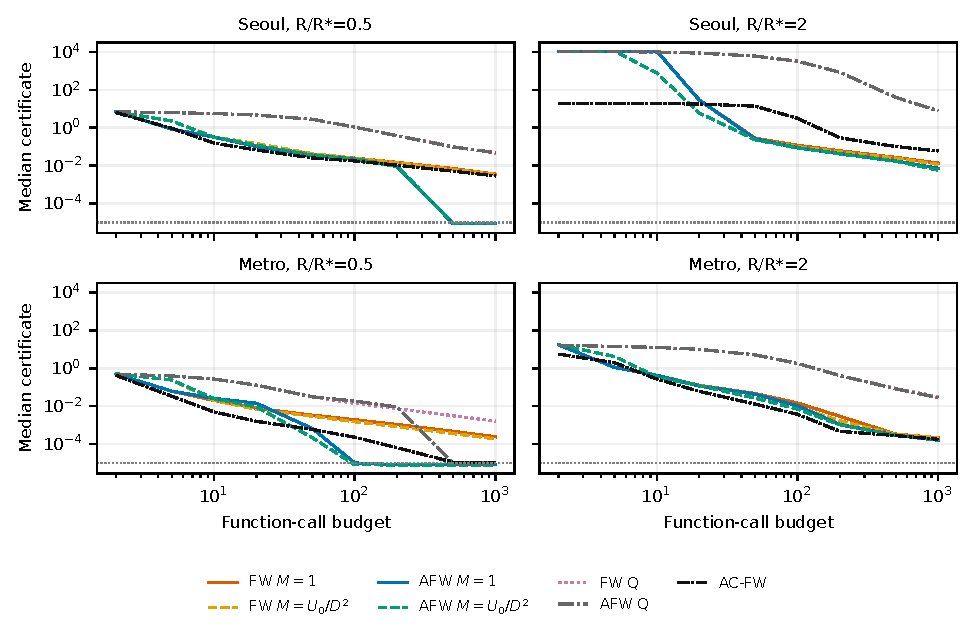
\includegraphics[width=\textwidth]{figures/count_comparators.pdf}
\caption{Median scalar certificates over all distinct vertices at
function-call budgets. Curves include failed runs and charged AC-FW
preprocessing; completed runs are carried forward. The dotted horizontal
line is $10^{-5}$. BT has no curvature inputs, Q receives analytic
$H_0,H_1$. These are paired finite cases, not confidence bands for a
population of problems.}
\label{fig:counts}
\end{figure}

At the active radii, both AFW-BT initializations certify every start at
1000 function calls. FW-BT certifies none on Seoul and only 2/24 or
3/24 on Metro. AC-FW obtains 13/24 active Metro successes and none
on active Seoul. The known-curvature AFW-Q succeeds on all active
Metro starts but none on active Seoul, illustrating conservatism of
the analytic curvature parameters. At the interior radii no method in
this seven-method scalar-certificate comparison reaches the target
within 1000 function calls. End-of-cap results and censored call
medians are reported separately in Table~\ref{tab:counts}.

The references separate remaining error from stopping lag. At the
interior Metro radius, all 24 starts of each BT variant have numerical
reference error upper bound at most $10^{-5}$ by the original endpoint,
but FW has no scalar-certificate successes and AFW has only 6/24 or
7/24. On interior Seoul, the corresponding reference-error condition
holds for 12/30 and 18/30 AFW starts, while neither scalar BT variant
stops. An unsuccessful certificate is therefore not equivalent to a
large remaining primal error.

\subsection{Controlling initialization and objective units}
A separate $2\times2$ study controls the original point versus the
compulsory LMO vertex, and AC versus BT updates. All four cells pay
the same two-source preprocessing, retain both tangent bounds, and
start their first trial at the same secant curvature. Only AC/vertex
is the native published comparator; the other cells isolate factors.
The study contains 280 runs on 70 earlier matched cases and introduces
no new datasets. Table~\ref{tab:init} shows all three planted active
families, including the unfavorable scaled family. Their construction
and the active-face slack identity appear in Appendix~\ref{app:protocol}.

\begin{table}[htbp]
\centering\small
\caption{Starting-point control on three planted active families, ten matched instances each. Counts are certified starts at 1000 function calls. O/V: original point/compulsory initial LMO vertex. The last column is the descriptive paired median BT-V/AC-V certificate ratio and 95\% percentile-bootstrap interval, not a speedup estimate.}
\label{tab:init}
\begin{tabular}{lrrrrl}
\toprule
Family & AC-O & AC-V & BT-O & BT-V & Ratio [interval] \\
\midrule
active & 1 & 10 & 0 & 10 & 1.049 [0.935, 1.257] \\
active\_scaled & 0 & 0 & 0 & 0 & 1.530 [0.822, 1.750] \\
active\_highdim & 6 & 8 & 2 & 8 & 1.231 [0.798, 2.117] \\
\bottomrule
\end{tabular}
\end{table}

On the active family, changing the starting point raises successes
from 1 to 10 for AC and from 0 to 10 for BT. The descriptive
BT/AC certificate-ratio interval from the vertex includes one.
The scaled family remains unsolved by all four controls. Thus the
earlier vertex-start comparison does not isolate an update-rule benefit.

Objective units provide another control. Under $\widetilde f=af+b$,
$a>0$, scaling $M$ and $\varepsilon$ by $a$ preserves the exact
iterates, trials and stopping index, since $G,U,L$ scale together.
Thus $M=U_0/D^2$ is automatically equivariant; fixing its numerical
value instead changes effective initialization. A separate real-data
radius/scale study verifies the counts in all 60 paired scale
comparisons for each certificate-initialized method. This elementary
property does not establish a faster algorithm.

\subsection{Causal stopping controls on fixed BT paths}
We repeat the 432 original BT paths from the count-data study, with
exactly matching original endpoints and oracle counts. Five causal
monitors give 2160 dependent stopping profiles. Disjoint blocks of
$K=8,32,128$ paid affine tangents provide a lower bound using one
additional full LMO per completed block; the scalar envelope is
retained. A separate standard control receives $\mu=0.01$ and uses
$f-\norm{\nabla f}^2/(2\mu)$ as a lower bound. Appendix~\ref{app:monitors}
proves validity and isolated oracle accounting; block sizes are fixed
before outcomes and no monitor reads the reference.

\begin{table}[htbp]
\centering\small
\caption{Isolated causal controls on 432 exactly repeated BT paths, giving 2160 dependent profiles. Counts use each profile's first stop or the original cap. More LMOs compares total direction plus certificate LMOs with scalar. Known $\mu$ receives the analytical ridge coefficient; blocks do not.}
\label{tab:monitors}
\begin{tabular}{lrrr}
\toprule
Profile & Certified & Earlier prefix & More total LMOs \\
\midrule
scalar & 129 & 0 & 0 \\
block\_8 & 129 & 0 & 432 \\
block\_32 & 129 & 0 & 425 \\
block\_128 & 129 & 0 & 380 \\
known\_mu & 226 & 110 & 0 \\
\bottomrule
\end{tabular}
\end{table}

None of the tested blocks gives an earlier stop. The known-$\mu$
control gives 226 successes instead of 129 and 110 earlier prefixes,
with no extra LMOs but additional model information. On interior
Metro each BT variant now reaches 24/24 successes by the original
endpoint; both AFW variants do so within 1000 function calls.
Interior Seoul remains difficult: AFW obtains only 4/30 or 10/30
successes by the endpoint and none at 1000 function calls.
These controls neither establish adaptation to unknown strong convexity
nor evaluate the exact averaged-gradient Fenchel dual in~\cite{pedregosa}.
They show that observable stopping cost is a separate practical issue.
